\subsection{Элементы теории устойчивости}
\begin{equation}
\label{stable}
\dv x = f(\v x), \, \v x \in \R^n, \, \v f \in C^1: \R^n \rightarrow \R \quad \v x(t) = \v x(t, \v x(0)) \text{ --- начальные условия.}
\end{equation}\

\begin{df}
$ \v x = \v x_0 $ --- положение равновесия \eqref{stable}, если $\v f(\v x_0) = 0$ ($\v x(t, \v x_0 \equiv \v x_0$) $\v x_0 = 0$ без ограничения общности. 
\end{df}

\begin{df}
Равновесие \eqref{stable} устойчиво по Ляпунову, если для любого $\varepsilon > 0$ существует $\delta > 0 $, что любое решение с начальными условиями в $\delta$-окрестности равновесия существует при всех $t > 0$ и находится в $\varepsilon$-окрестности.
\[
	\forall \varepsilon > 0 \ \exists \delta > 0 \ \abs{\v x(0)} < \delta \Rightarrow \abs{\v x(t)} < \varepsilon, \ \forall t > 0.
\]
\end{df}

\begin{df}
$\v x = 0$ --- неустойчивое, если
\[
	\exists \varepsilon > 0 \ \forall \delta > 0 \ \exists \v x(0), t_1 > 0: \abs{x_0} < \delta \ \abs{\v x(t_1, \v x_0)} > \varepsilon
\]
\end{df}

\begin{df}
$\v x = 0$ --- устойчиво асимптотически, если
\begin{enumerate}
\item $\v x = 0$ --- устойчиво,
\item $\lim\limits_{t \rightarrow +\infty} \v x(t, \v x(0)) = 0$. 
\end{enumerate}
\end{df}

\subsection{Прямой метод Ляпунова}
\begin{fl*}
& V(x) &\\
& \dot V = \pd{V}{\v x} \dv x = \pd{V}{\v x} \v f &\\
\end{fl*}

\begin{df}
$\dot V$ --- производная функции $V$ по времени вдоль решения \eqref{stable}.
\end{df}

\begin{teo}[Ляпунова об устойчивости]
Если существует гладкая функция $V(x)$ определенная в $\varepsilon$-окрестности равновесия $x = 0$ системы \eqref{stable}, удовлетворяющая следующим условиям:
\begin{enumerate}
\item 
\[
	V(0) = 0, \ \forall x \in U_\varepsilon \setminus \{ 0 \},
\]
\item
\[
	\dot V \leqslant 0 \ \forall \v x \in U_\varepsilon,
\]
\end{enumerate}
то $x = 0$ --- устойчиво по Ляпунову.
\end{teo} 
\begin{proof}
\begin{fl*}
& 1) \forall \varepsilon > 0, \ \exists \sigma = \min V(\v x), \abs{ \v x } = \varepsilon &\\
& 2) V \in C^1 \Rightarrow \exists \delta: V(\v x) < \sigma \ \forall \v x : \abs{\v x} < \delta &\\
& 3) \forall \v x_0: \ \abs{\v x_0} < \delta \ V(\v x(t)) < \sigma \Rightarrow \abs{\v x_0(t)} < \varepsilon \quad (\v x_0(t) = \v x(t, \v x_0)) &\\
\end{fl*}
\begin{figure}[H]
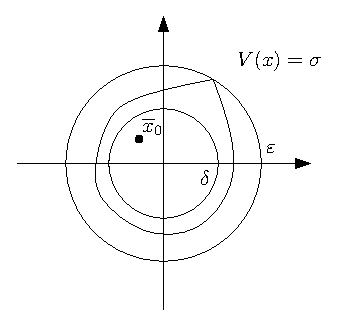
\includegraphics{2_1.eps}
\end{figure}
\end{proof}

\begin{ntc}
\begin{fl*}
& 1) V(0) = 0, V(\v x) > 0 \ \forall \v x \in U_\varepsilon \setminus \{0\} \Rightarrow \text{ $V$ --- положительно определенная функция в 0}. &\\
& 2) V(0) = 0, V(\v x) < 0 \ \forall \v x \in U_\varepsilon \setminus \{0\} \Rightarrow \text{ $V$ --- отрицательно определенная функция в 0}. &\\
& 3) V(0) = 0, V(\v x) \geqslant (\leqslant) \: 0 \ \forall \v x \in U_\varepsilon \setminus \{0\} \Rightarrow \text{ $V$ --- знакопостоянная функция в 0}. &\\
\end{fl*}
\end{ntc}

\begin{xmp}~\\
$V(x_1, x_2) = x_1^2 + x_2^2$ --- положительно определена в $x_1 = x_2 = 0$ \\
$V(x_1, x_2) = x_1^2$ --- не является положительно определенной в $x_1 = x_2 = 0$
\begin{figure}[H]
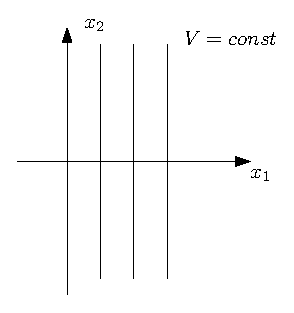
\includegraphics{2_2.eps}
\end{figure}
\end{xmp}

\begin{ntc}
Если в условии теоремы Ляпунова в условии $2)$ поставить строгое неравенство, устойчивость станет асимптотической.
\end{ntc}

\begin{teo}{Барбашина-Красовского}
Если $\exists V(x) \in C^1 : U_\varepsilon \rightarrow \R$, то
\begin{enumerate}
\item 
\[
	V(0) = 0 \ V(\v x) > 0 \ \forall \v x \in U_\varepsilon \setminus \{ 0 \},
\]
\item
\[
	\dot V \leqslant 0 \  \forall \v x \in U_\varepsilon,
\]
\item множество $\{\v x : \dot V (\v x) = 0\}$ не содержит целиком решения системы \eqref{stable}, кроме равновесия $\v x = 0 \Rightarrow \v x = 0$ --- установившееся асимптотически.
\end{enumerate}
\end{teo}

\begin{ntc}
Если $\dot V < 0$, то $\{ x: \dot V = 0 \} = \{ 0 \}$.
\end{ntc}
\begin{proof}
Пусть $\v x = 0$ установившееся, но не асимптотическое, т.е. 
\begin{fl*}
& I)\  \exists \v x_0(t) \ \abs{\v x_0 (t)} < \varepsilon, \ \v x_0 \not \rightarrow 0 \text{, т.е.} &\\
& \exists \delta, \{t_k\}, \ t_{k + 1} > t_k \ \delta < \abs{\v x_0(t_k)} < \varepsilon &\\
& II)\ \exists \{k_s\} \  \v x_s = \v x_0(t_{k_s}) \xrightarrow{s \rightarrow +\infty} \v x_* &\\
& \abs{\v x_s} > \delta \Rightarrow \abs{\v x_*} > \frac{\delta}{2} &\\
& III)\ V(\v x_0(t)) &\\
& 1),\; 2) \Rightarrow \exists V = \lim_{t \rightarrow + \infty} V(x_0(t)) &\\
& V \in C^1 \Rightarrow V = V(\v x_*) &\\
\end{fl*}
\begin{figure}[H]
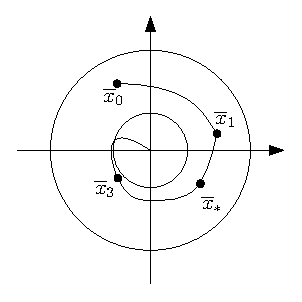
\includegraphics{2_3.eps}
\end{figure}
\begin{fl}
\label{triplesec}
& \boxed{\forall t \ V(\v x_0(t)) \geqslant V} &\\
\end{fl}
\begin{fl*}
& IV)\ \text{Рассмотрим} \v x_s(t) = \v x(t, \v x_s) = \v x_0(t + t_{k_s}, \v x_0) &\\
& V)\ \v x_*(t) = \v x(t, \v x_*) &\\
& V(\v x_*) = V, \ 2),\; 3) \Rightarrow \exists t^*: \underbrace{V(\v x_*(t_*))}_{V_*} < V &\\
& VI)\ V \text{ --- непрерывная б.т. } \v x_*(t_*) &\\
& \forall \varepsilon_1 > 0 \ \exists \delta_1 > 0 \ \forall x \ \abs{\v x - \v x_*(t_*)} < \delta_1 \Rightarrow \abs{V(\v x) - V(x_*(t_*))} < \varepsilon_1 &\\
& \text{Решения \eqref{stable} непрерывно и зависит от начальных условий ($t < \infty$)} &\\
& \forall \varepsilon_2 > 0 \ \exists \delta_2 > 0 \ \forall x \ \abs{\v x - \v x_*(t_*)} < \delta_2 \Rightarrow \abs{\v x(t_*) - x_*(t_*)} < \varepsilon_2 &\\
& \forall \varepsilon_3 > 0 \ \exists s: \abs{\v x_s - x_*} < \varepsilon_3 \forall s > S &\\
& \varepsilon_1 = V - V_* > 0 \rightarrow S: \ \abs{V(\v x_s(t_*)) - \underbrace{V(\v x_*(t_*))}_{V_*}} < V - V_* &\\
& V(\v x_s(t_*)) - V_* < V - V_* \text{ --- противоречие с \eqref{triplesec}}
\end{fl*}
\end{proof}

\begin{teo}[Красовского]
$\exists V \in C^1: U_\varepsilon \rightarrow \R$ и область $\Omega$:
\begin{enumerate}
\item $V(0) = 0,\  V(\v x) > 0\  \forall \v x \in U_\varepsilon \cap \Omega$ \\
$\v x = 0 \in \partial \Omega, V(\v x) = 0 \ \forall \v x \in \partial \Omega$
\item $\dot V \leqslant 0 \ \forall \v x \in U_\varepsilon \cap \Omega$
\item $\{ \v x: \dot V = 0 \} \Rightarrow \v x = 0$ --- неустойчивое.
\end{enumerate}
\end{teo}
\begin{proof}
\begin{flalign*}
& \exists \v x = 0 \text{ --- устойчивое, т.е. } &\\
& \forall \varepsilon > 0 \exists \delta > 0: \abs{\v x_0} < \delta \Rightarrow \abs{\v x_0(t)} < \varepsilon &\\
& 1), 2) \Rightarrow \exists \delta: \abs{\v x_0(t)} > 0 \Rightarrow \exists\{ x_s \} \rightarrow \v x_*, &\\
& V(\v x_s(t)) \leqslant V(\v x_*) = V &\\
& \v x_*(t),\  3) \Rightarrow \exists t_* > 0: (\v x_*(t_*)) > V \text {--- противоречие как в предыдущей теореме} &\\
\end{flalign*}
\begin{figure}[H]
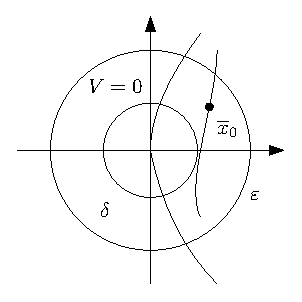
\includegraphics{2_4.eps}
\end{figure}
\end{proof}

\begin{ntc}
$\dot V > 0$ --- теорема Четаева.
\end{ntc}

\begin{xmp}[Волчок Эйлера]
\begin{flalign*}
& \begin{cases}
	A\dot p + (C - B)qr = 0 \\
	B\dot q + (A - C)rp = 0 \\
	C\dot r + (B - A)pq = 0 \\
\end{cases} \quad \begin{array}{l}
	p = \omega \\
	q = r = 0 \\
	p' = p - \omega \\
\end{array}
\Rightarrow
\begin{cases}
	A\dot p' = (B - C)qr \\
	B\dot q = (C - A)r(p' + \omega) \\
	C\dot r = (A - B)q(p' + \omega) \\
\end{cases} &\\
& 2T = A(p' + \omega)^2 + Bq^2 + Cr^2 = Ap'^2 + Bq^2 + Cr^2 + 2Ap'\omega + A\omega^2 \quad | \cdot A &\\
& k^2 = A^2p'^2 + B^2q^2 + C^2r^2 + 2A^2p'\omega + A^2\omega^2 &\\
& 2TA - k^2 = B(A - B)q^2 + C(A - C)r^2 + 0\cdot p^2 &\\
& V = (2TA - k^2) + (2T - A\omega^2)^2 = B(A - B)q^2 + C(A - C)r^2 + 4A^2\omega^2(p')^2 + O_4(p',\; q,\; r) &\\
& A > B,\; A > C &\\
& \text{Т.к. все слагаемые больше 0, } O_4 \text{ мало в окрестности } 0. &\\
& \exists{u_\varepsilon}: V > 0, \forall (p',\; q,\; r) \in U_\varepsilon,\; V \geqslant 0 |_{p' = r = q = 0}, \dot V = 0 \Rightarrow \text{ равновесие устойчтво.}
\end{flalign*}
\end{xmp}